\documentclass[12pt]{article}
\usepackage[margin=0.5in]{geometry}
\usepackage{amsmath}
\usepackage{amssymb}
\usepackage{graphicx}
\usepackage{silence}
\WarningsOff[latex]
\usepackage{float}
\graphicspath{ {./pics/} }
\linespread{1.2}
\newcommand{\code}{\texttt}
\usepackage{csquotes}
\usepackage{algorithm}
\usepackage{algpseudocode}
\usepackage{algorithmicx}

\begin{document}
\subsection*{Q1.}
Since we use simple uniform hashing, the average number of elements that hash to the same array would be \(\alpha = \frac{n}{m}\), where \(n\) is the total number of elements in the hash table, and \(m\) is the number of slots.

\paragraph{(a).} Given that we use sorted arrays as the chaining components for the hash table:\\ On average, the time complexity for search would be \(O(1+\log(\alpha))\),  Here, \(O(1)\) is the time taken to compute \(h(k)\), and \(O(\log(\alpha))\) is the time to search for the key inside the array at slot \(h(k)\). We achieve logarithmic runtime as we could perform binary search on the sorted array, since arrays allow random access. However, if \(\alpha\) is very small, we would not have much benefit from the usual way of using linked list as the chaining component (runtime being \(O(1+\alpha)\)). But in the case that \(n \gg m\), then the runtime would improve.

\paragraph{(b).} Given that we need to run a merge sort every time we insert an element:\\
On average, the time complexity for insertion would be \(O(1+\alpha\log(\alpha))\), where \(O(1)\) is the time to compute \(h(k)\), and \(O(\alpha\log(\alpha))\) is the time to perform the merge sort on the array at slot \(h(k)\). If we do not keep track of the current number of elements in the array, then we also have an additional cost of \(O(\alpha)\) to search to the end for an empty spot, otherwise it would just take \(O(1)\) time to append. Yet in the end, the insertion time would be worse than the original scheme of using linked lists, as it only costs \(O(1)\) time to add the key to the front of the linked list.

\paragraph{(c).} Deletion with sorted arrays would remain the same as using linked lists, i.e. \(O(1 +\alpha)\). \(O(1)\) is the time to compute \(h(k)\), and \(O(\alpha)\) is the total cost for deletion. To delete, we first need to search for the key, so it takes \(O(\log(\alpha))\) to perform binary search, then remove the key by shifting all elements greater than the deleted key one slot to the left. In the worst case, the deleted key is the first element, so we need to shift all the remaining elements, which is \(O(\alpha)\). Since \(O(\log(\alpha)) \in O(\alpha)\), we have the overall cost for search-delete-shift as \(O(\alpha)\). With linked lists, deletion is also \(O(\alpha)\). We need to traverse the list to search for the previous element of the target, then change its pointer to the next (\(O(1)\)), and free memory for the target(\(O(1)\)). In the worst case, the target is the last element, so we require \(O(\alpha)\).

\subsection*{Q2.}
His claim is not correct for all situations. There is no guarantee that the leaves of a complete binary tree are on the same level. There could be missing right-most nodes on the last level. As illustrated in Figure 1, all internal nodes of a complete binary tree have two children, but the leaves here are not on the same level, meaning that if we color all nodes as black, the number of black nodes from root to a leaf is not the same for all paths. This violates the red black tree property:
\begin{displayquote}[][]
     For each node, all paths from this node to each of its leaves contain the same number of black nodes.
\end{displayquote}
Hence, it is not a red black tree in this case.
\begin{figure}[H]
     \centering
     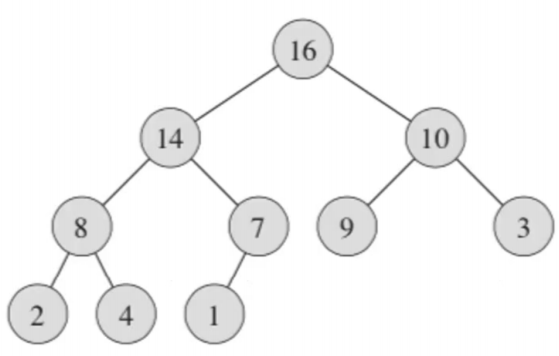
\includegraphics[scale =0.8]{q2a.png} 
     \caption{missing right-most nodes}
\end{figure}

\noindent However, if we have a perfect binary tree, which is a complete binary tree with all leaves on the same level (assuming leaves are nil), then it is valid red black tree:
     \begin{enumerate}
          \setlength \itemsep{0em} 
          \item the root is black
          \item leaves are black nils
          \item there is no consecutive red nodes along any path since there are no red nodes at all
          \item all paths from a node to its leaves contain the same number of black nodes.
     \end{enumerate}

\subsection*{Q3.}
An avl tree is a self balancing binary search tree that has the property that, for any node \(x\) in the tree, \(x\) has at most two children, and \(x.left.key \leq x.key \leq x.right.key\). Although for an avl tree, we might need rotation for insertion and deletion operations in order to maintain the balance factor, we still guarantee that the bst property holds. So the node with the minimum key is the left-most node in the tree. We could find it by traversing down the tree from the root, and always choosing the left subtree to traverse, until we find the left subtree to be nil, then the current node contains the minimum key. Similarly, the node with the maximum key is the right-most node in the tree. Beginning from the root, we always traverse the right subtree, until the right subtree is nil, then the current node contains the maximum key. 

\subsection*{Q4.}

\subsection*{Q5.}
\paragraph{(a).}
First, we simplify the problem into a longest decreasing subsequence (LDS) problem by sorting. We sort based on the first parameter, i.e. radius, in the descending order. This ensures that we could choose a longest decreasing sequence out of the original unsorted \(n\) boxes, by simply finding the LDS of the sorted sequence. Note that here we cannot solve the LDS based on height purely, since in the case where radius are the same and height are in the descending order, we might mistakenly contribute boxes of the same radius to the LDS. We could avoid this by also sorting based on height, in the ascending order, for the boxes of the same radius, and then find the LDS based on height only.
Now we can find the LDS by dynamic programming. \\
\textbf{Sub-problems:} The sub-problems are LDS of the prefixes of the sorted sequence, and the LDS is ended with the last element of the prefix. We also find the length of such LDS. A solution to the original problem would be a longest sequence among all solutions to the sub-problems.\\
\textbf{Relation between sub-problems:}
\begin{itemize}
     \setlength \itemsep{0em} 
     \item On LDS:\\
     Suppose \(P_i = \langle(r_1,h_1), (r_2, h_2), \hdots, (r_i, h_i)\rangle\) is the sequence that is sorted as described above, then a LDS that ends with the element \((r_i, h_i)\), is built from a LDS that ends with \((r_k, h_k)\) for \(k \in [1, i-1]\) where \(h_k > h_i\). There could be multiple \(k\)'s that form the LDS of \(P_i\). Or if such \(k\) does not exist, then the LDS is \(\langle(r_i, h_i)\rangle\). Expressed as a formula, 
     \begin{equation*}
          \text{LDS(\(P_i\))} = \text{longest}(\langle(r_i, h_i)\rangle, \underset{\substack{k \in [1, i-1] \\ h_k > h_i}}{\text{longest}}(\text{LDS(\(P_k\))} + \langle(r_i, h_i)\rangle)
     \end{equation*}
   Here \('+'\) is the concatenation of two sequences, and \(P_k\) is the slice \(P_i\)[\(1 .. k\)].
     \item On the length of LDS:
     \begin{equation*}
          dp[i] = 
          \begin{cases}
               1 & i = 1 \\
               \max (1, \displaystyle\max_{\substack{k \in [1, i-1] \\  h_k > h_i}}(1 + dp[k])) & i > 1
          \end{cases}
     \end{equation*}
     \(dp[i]\) is the length of the LDS of \(P_i\) and the last element of the LDS is \((r_i, h_i)\)
\end{itemize}
 
\paragraph{(b)} Let \(P\) denote the input list \([(r_1,h_1), (r_2,h_2), \hdots, (r_n,h_n)]\). In the following psuedocode, we access the \(i^{th}\) element in \(P\) by \(P[i]\), and access \(r_i\) by \(P[i].r\) and  \(h_i\) by \(P[i].h\).
\begin{algorithm}[H]
     \caption{Bottom-up Longest Strictly Decreasing Sequence(\(P\))}
     \begin{algorithmic}[1]
     \State let \(dp[1..n]\) be an empty array \Comment{\(dp[i]\) stores the length of LDS(\(P_{sorted} [1 .. i]\)) that ends with \(P_{sorted}[i]\)}
     \State let \(prev[1..n]\) be an empty array \\ \Comment{\(prev[i]\) stores the index of the second last element of LDS(\(P_{sorted} [1 .. i]\))}
     \State \textbf{MergeSort} (\(P, 1, n\)) \Comment{in descending order based on \(r\)}
     \For {\(i = 1\) to \(n\)}
          \State \(dp[i] = 1\)
          \State \(prev[i] = i\) \Comment{prev of the first element is set to be itself}
          \For {\(k = 1\) to \(i-1\)}
               \If{\(P_{sorted}[k].h > P_{sorted}[i].h\) \textbf{and} \(1 + dp[k] > dp[i]\)} 
                    \State \(dp[i] = 1 + dp[k]\)
                    \State \(prev[i] = k\)
               \EndIf
          \EndFor
     \EndFor
     \State int \(l = 0\)
     \State int \(idx\) 
     \For{\(i = 1\) to \(n\)}
          \If {\(dp[i] > l\)}
               \State \(l = dp[i]\) \Comment{\(l\) is the maximal length of the output sequence}
               \State \(idx = i\) \Comment{\(idx\) is the index in \(P_{sorted}\) of the last element in the output sequence}
          \EndIf
     \EndFor
     \State let \(O[1..l]\) be the output sequence
     \While {\(idx \neq prev[idx]\)}
          \State \(O[l] = P_{sorted}[idx]\)
          \State \(idx = prev[idx]\)
          \State \(l = l - 1\)
     \EndWhile
     \State \(O[l] = P_{sorted}[idx]\)
     \State \Return \(O\)
     \end{algorithmic}
\end{algorithm}
\noindent The Merge function for the MergeSort is modified as follows
\begin{algorithm}[H]
     \caption{Merge in descending order (\(P, p, q, r\))}
     \begin{algorithmic}[1]
          \State \(n_1 = q-p+1\); \(n_2 = r-q\)
          \State let \(L=[1 .. n_1 + 1]\) and \(R=[1.. n_2 +1]\)
          \For {\(i = 1\) to \(n_1\)}
               \State \(L[i] = P[p+i-1]\) \Comment{copy of lower subarray}
          \EndFor
          \For {\(i = 1\) to \(n_2\)}
               \State \(R[i] = P[q+i]\) \Comment{copy of upper subarray}
          \EndFor
          \State \(L[n_1+1] = \infty\); \(R[n_2+1] = \infty\)
          \State \(i = 1\); \(j = 1\)
          \For {\(k = p\) to \(r\)}
               \If {\(L[i].r > R[i].r\)} \Comment{\textbf{modification from here onwards}}
                    \State \(P[k] = L[i]\)
                    \State \(i = i + 1\)
               \ElsIf {\(L[i].r = R[i].r\)}
                    \If {\(L[i].h \leq R[i].h\)}
                         \State \(P[k] = L[i]\)
                         \State \(i = i + 1\)
                    \Else 
                         \State \(P[k] = R[i]\)
                         \State \(j = j + 1\)
                    \EndIf
               \Else
                    \State \(P[k] = R[i]\)
                    \State \(j = j + 1\)
               \EndIf
          \EndFor
     \end{algorithmic}
\end{algorithm}

\paragraph{(c).} Time complexity is \(O(n^2)\). The merge sort takes \(O(n\log n)\). The computation of LDS that ends with each element of \(P_{sorted}\) requires two for loops (line \(3-12\)). The outer loop iterates through each element of the sorted sequence (\(n\) times), and the inner loop searches through all previous computed LDS. The total number of operations at line \(6\) is therefore \(\sum_{i=1}^n i-1 = \frac{n(n-1)}{2} = O(n^2)\). The loop body is just constant time operations, so the total cost is \(O(n^2)\). Line \(15-20\) searches for the longest sequence among all LDS sub-problems. This takes another \(O(n)\) time. Line \(21-28\) outputs the sequence by tracing from the last element to the first. This takes at most \(O(n)\) time since the sequence is at most of length \(n\). The total time complexity would therefore be \(O(n\log n) + O(n^2) + O(n) + O(n) = O(n^2)\).

\subsection*{Q6.}
\paragraph{(a).} Given that \(k_i\) is the number of proposals for the \(i^{th}\) approach, and \(m_{ij}\) is the funding requested for the \(j^{th}\) proposal for the \(i^{th}\) approach, where \(j \in [1, k_i]\). The following algorithm relies heavily on the assumption that all \(m_{ij}\) are integer numbers, and assuming this is allowed in the problem specification. We would use a \(dp\) table to compute the choices of proposals. In the following psuedocode, entry \(dp[i][j]\) is a pair of values \(\langle x,y\rangle\) where \(x\) is a funding sum (potentially many possibilities) requested by the previous (\(i-1\)) approaches, given that \(j\) is the exact funding requested by all \(i\) approaches; and the second value \(y\) is the corresponding index of the proposal for the \(i^{th}\) approach such that \(x\) + \(m_{iy}\) = \(j\). If there is no set of proposals for the first \(i\) approaches that sum to \(j\) exactly, \(dp[i][j]\) would be \(\langle 0,0\rangle\). The reason for keeping the fund sum of the previous \((i-1)\) proposals is to back trace the selected proposals at the end.
\begin{algorithm}[H]
     \caption{Set of proposals (n, F, m)}
     \begin{algorithmic}[1]
          \State let \(dp[1..n][1..F]\) be an empty table \Comment{assume all entries are initialized to \(\langle 0,0\rangle\)}
          \For {\(j = 1\) to \(k_1\)}
               \State \(dp[1][m_{1j}] = \langle 0,j \rangle\) \Comment{initialize the pair for the first approach}
          \EndFor
          \For {\(i = 1\) to \(n-1\)}
               \For {\(j=1\) to \(F\)}
                    \If {\(dp[i][j] \neq \langle 0,0 \rangle\)}
                         \For {\(y = 1\) to \(k_{i+1}\)}
                              \If {\(j + m_{(i+1)y} < F\)}
                                   \State \(dp[i+1][j+m_{(i+1)y}] = \langle j,y \rangle\)
                              \EndIf
                         \EndFor
                    \EndIf
               \EndFor
          \EndFor
          \State let \(seqProposals[1..n]\) be the indices of the selected proposals
          \State let \(reqFund[1..n]\) be the fund requested by the selected proposals
          \State let \(totalFund\) be the total fund distributed
          \For {\(j = F\) to \(1\)}
               \If {\(dp[n][j] \neq \langle 0,0 \rangle\)} \Comment{check the last row for the maximum fund distributed}
                    \State \(totalFund = j\)
                    \State \(sum = j\)
                    \For {\(i = n\) to \(1\)} \Comment{back trace the sequence}
                         \State \(seqProposals[i] = dp[i][sum].second\)
                         \State \(reqFund[i] = m_{i(seqProposals[i])}\)
                         \State \(sum = dp[i][sum].first\)
                    \EndFor
                    \State \textbf{break}
               \EndIf
          \EndFor
          \State \Return \(totalFund\), \(seqProposals\), \(reqFund\)
     \end{algorithmic}
\end{algorithm}
\paragraph{(b).} Time complexity is \(O(F \times \sum_{i=1}^{n} k_i)\). In line \(5-15\), there are \(3\) for loops. The for loop at line \(5\) and for loop at line \(8\) sums to be \(\sum_{i=1}^{n-1} k_{i+1} = \sum_{i=2}^{n} k_{i} = O(\sum_{i=1}^{n} k_{i})\). This is then multiplied by \(F\) because of the for loop at line \(6\). The loop body is constant time operation, so line \(5-15\) is \(O(F \times \sum_{i=1}^{n} k_i))\). The initialization cost at line \(2-3\) costs another \(O(k_1)\) operations, and to output the final set of proposals at line \(19-30\), we have to traverse the last row of the dp table, which would at most iterate \(F\) times if there is no solution. If there is a solution, then we have another \(O(n)\) operations to trace backwards the sequence of proposals. Hence, in sum there should be \(O(F \times \sum_{i=1}^{n} k_i) + O(k_1) + O(F) + O(n)\), which is dominated by \(O(F \times \sum_{i=1}^{n} k_i)\). Notice that if we also count the initialization cost at line \(1\), which is \(O(n \times F)\) as the dimension of the table is \(n \times F\), in the end we still get \(O(F \times \sum_{i=1}^{n} k_i)\) as the time complexity since \(n \leq \sum_{i=1}^{n} k_i)\).

\paragraph{(d).}
Empirical analysis:
\begin{figure}[H]
     \centering
     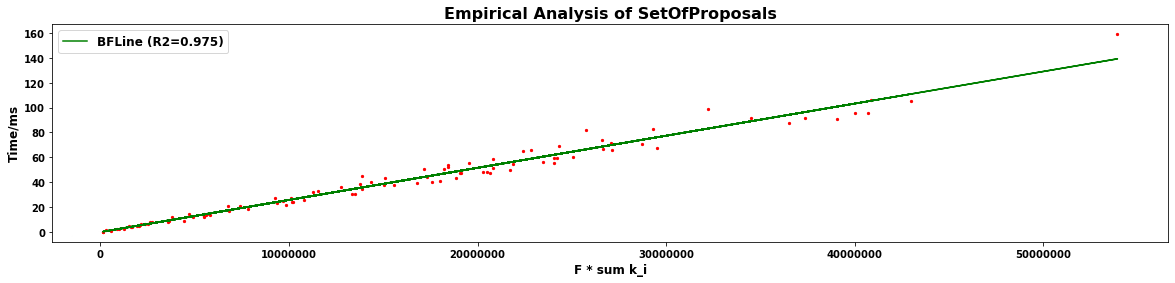
\includegraphics[width = \textwidth]{q6d.png}
\end{figure}
\noindent This plotted graph is based on a data set of 100 samples. We observe a linear relationship between the time taken in \(ms\), and the number  (\(F \times \sum_{i=1}^n k_i\)). The best fit line has a \(R^2\) coefficient of \(0.975\), which means that the linear model fits the data set well. Hence, we could conclude that the time complexity of the algorithm is some constant times \(F \times \sum_{i=1}^n k_i\), and hence there is \(c, n_0 > 0\) such that \(T(n) \leq c(F\times \sum_{i=1}^n k_i)\) for all \(n \geq n_0\). Time complexiy is therefore \(O(F \times \sum_{i=1}^n k_i)\) and the empirical analysis matches with our theoretical analysis. 

\end{document}